\cotefile{8}
\scanpage{17}
% sheet: cancelled_draft
% archive sheet number: 16
% Three long oblique pencil strokes cross the two sections.
% @ text / top, item 3
\deleted{-- \textcircled{3} Indétermination dans ces données, pour $(\deleted{\unsure{G}}M,T)$ (i.e. $G$) fixée.}

% @ text / upper third, body of item 3
\deleted{La catégorie des données \deleted{$\unsure{T}$\illegible{1}} en question est \deleted{\illegible{1}} ``un torseur'' sous la catégorie des torseurs sous $\mu_2$ sur $A'$, donc l'ensemble des classes d'isomorphie de ces structures est \inserted{un torseur sous} $H^1(A^{\deleted{\unsure{*}}},\mu_2)\simeq\prod_p Q_p^*/Q_p^{*2}$, \inserted{\unsure{pr. direct|pr. dir.} local rel. à \unsure{l'un des ss-gpes|l'un des sous-gpes|l'un des deux-gpes} $\mathbb Z_p^*/\mathbb Z_p^{*2}$} l'ensemble des autom. d'un objet de la catégorie est $H^0(A',\mu_2)=\prod_p(\mathbb Z/2\mathbb Z)$}
% slanted
\margin{modulo \unsure{mes|une} \unsure{légers renforcements de la|ligne renforcée de la} donnée à l'\unsure{$\infty$}}

% @ text / middle, item 4
\deleted{\textcircled{4} Rigidité de $M$ pour les structures envisagées.}

% @ text / middle, before equivalence
\deleted{Soit $(M',T')$ muni des \deleted{\unsure{mêmes}} données \inserted{suppl.} que $(M,T)$. On se demande de déterminer la catégorie des équivalences}

% @ display / middle
\deleted{\[
(M,T,\overbrace{T_{A'},u_{A'}}^{t_{A'}},t_\infty,t_p)\longrightarrow (M',T'\ \text{etc}\qquad)
\]}

% @ text / middle to lower third
\deleted{\deleted{\unsure{Elles|Ils|Elle}} \inserted{Cette catégorie est vide, \uuline{ou}} forme un torseur sous la catégorie des torseurs sous $\mu_2$ sur $Q$, \uline{munis} d'une trivialisation \deleted{\unsure{de}\illegible{1}} au dessus \deleted{\unsure{de}} $A$. Cette dernière catégorie a comme \deleted{\unsure{ensemble}} \inserted{groupe} de \deleted{\unsure{d'id}} classes d'objet à isom près le groupe}

% @ display / lower middle
\deleted{\[
H^{1}(Q\ \mathrm{mod}\ A,\mu_2)\simeq {}_2(\unsure{J|\mathcal I}_Q)\simeq\bigl(\prod_p\mathbb Z/2\mathbb Z\bigr)/(\pm1)
\]}
\margin{qui a la puiss. du continu $\bigr]$}

% @ text / lower third, rigidity
\deleted{d'autre part cette catégorie est rigide $(H^0(Q\ \mathrm{mod}\ A,\mu_2)=0)$.}

% @ text / foot
\deleted{Comme l'image de $H^1(Q\ \mathrm{mod}\ A,\mu_2)$ dans $H^{1}(Q,\mu_2)$ est nulle, on voit que \uline{l'équivalence induite entre} $(M,T)$ \uline{et} $(M',T')$ \uline{est déterminée à isom. unique près}. Donc on peut identifier sans dommages $(M,T)$ et $(M',T')$}
\scanpage{18}
% archive sheet number: 17
% @ text / head
Soit $\omega$ sur $S_{\unsure{\mathrm{gros}|\mathrm{zar}}}$, avec $F_\omega,V_\omega$, on lui associe

% @ display / upper third, item 1 and its right-hand addition
\[
1^\circ)\qquad M=\varphi^*(\omega),\qquad F_M=\varphi^*(F_\omega),\quad V_M=\varphi^*(V_\omega)
\]
\margin{$M=\omega^{\unsure{\flat|b|p}}$}

% @ text / upper third, item 2
$2^\circ)$ Triangle
\margin{$\varepsilon^*(\Delta(M))=\Delta^*(\omega)$ complexe can. ext. de $\omega^{\unsure{\sharp|\flat|\prime}}$ par $\omega^\flat$}

% @ diagram / item 2, upper centre
\diagram{\begin{tikzcd}[ampersand replacement=\&,column sep=small,row sep=large]
\& {\mathcal T_2^{(\omega)}=[\omega\mathrel{\overset{V_\omega}{\text{---}}}\omega^{\flat}]} \arrow[dl,"1"'] \& \\
{\mathcal T(\omega)\ \unsure{\not\approx|\not\simeq}\quad\mathcal T_0^{(\omega)}=[\omega^{V}\mathrel{\overset{F_\omega}{\longrightarrow}}\omega]}
\arrow[rr] \& \& {\mathcal T_1^{(\omega)}=[\omega^{(p)}\mathrel{\overset{0}{\text{---}}}\omega^{(p)}]} \arrow[ul]
\end{tikzcd}}

% @ text / below triangle
déduit de $\omega$ $\bigl(\mathcal T_1^{(\omega)}=\Delta^*(\omega)\bigr)$

% @ text / middle, item 3
$3^\circ)$ Isom \uuline{can}
% @ display / middle, alpha
\[
\varphi^*(\mathcal T(\omega))\overset{\alpha_\omega}{\simeq}\mathcal T(\varphi^*(\omega))
\]

% @ display / middle, item 4
\[
4^\circ)\quad\text{L'\uline{identité}}\qquad
\mathcal T(\omega)_1\overset{\beta_\omega}{\simeq}\varepsilon^*\Delta^*(M))\simeq
[\omega^{\unsure{\sharp|N}}\mathrel{\overset{0}{\text{---}}}\omega^\flat]
\]

% @ text / centre, above rule
\uline{Question} Le foncteur
% @ display / assignment
\[
(\omega,F_\omega,V_\omega)\longmapsto
(\varphi^*(\omega),\varphi^*(F_\omega),\varphi^*(V_\omega),\mathcal T(\omega),\alpha_\omega,\beta_\omega)
\]
% @ text / immediately above rule
est-il pl. fidèle ?? L'est-il du moins sur la sous-catégorie des triples $(\omega,F_\omega,V_\omega)$ avec $F_\omega=0$ ?
\par\noindent\rule{\linewidth}{0.4pt}

% @ diagram / below rule, left brace
\diagram{\begin{tikzcd}[ampersand replacement=\&,column sep=large,row sep=small]
{\left\{\vphantom{\begin{matrix}a\\a\\a\end{matrix}}\right.} \& \varphi^*(\omega)\arrow[r,"u"] \& \varphi^*(\omega') \& \text{compatible avec }F,V \\
\& \mathcal T(\omega)\arrow[r,"v"] \& \mathcal T(\omega') \& \text{hom de nos triangles}
\end{tikzcd}}

% @ text / below brace, two qualifications
$v_1$ déterminé comme $\varepsilon^*(u)$ \qquad rendant commutatifs les diagrammes

$\varphi^*(v)$ déterminé par $u$ comme $\mathcal T(u)$

% @ diagram / lower right, upper square
\diagram{\begin{tikzcd}[ampersand replacement=\&,row sep=small]
\mathcal T_1(\omega)\arrow[r,"v_1"]\arrow[d,Rightarrow,"{\beta_\omega\,\unsure{\wr}}"',"1"] \& \mathcal T_1(\omega')\arrow[d,Rightarrow,"\beta_{\omega'}"]\\
\varepsilon^*\Delta^*(\varphi^*(\omega))\arrow[d,equal] \& \varepsilon^*(\Delta^*(\varphi^*(\omega')))\arrow[d,equal]\\
\Delta^*(\omega)\arrow[r,"\varepsilon^*(u)"'] \& \Delta^*(\omega')
\end{tikzcd}}

% @ diagram / bottom right, lower square
\diagram{\begin{tikzcd}[ampersand replacement=\&]
\varphi^*(\mathcal T(\omega))\arrow[r,dash,"\alpha_\omega","\sim"']\arrow[d,"\varphi^*(v)"'] \& \mathcal T(\varphi^*(\omega))\arrow[d,"\mathcal T(u)"]\\
\varphi^*(\mathcal T(\omega'))\arrow[r,dash,"\alpha_{\omega'}","\sim"'] \& \mathcal T(\varphi^*(\omega'))
\end{tikzcd}}
\scanpage{19}
% sheet: reused_typed
% hand: typed
% archive sheet number: 18
% @ text / head, right
Tribu n° 66

% @ text / head, centre
\uline{DÉCISIONS sur l' INTÉGRATION}

(Rédactions n° 446 et 447)

\mbox{-:-:-:-}

% @ text / upper third, first heading
\uline{La réédition d'Intégration V} (n° 446).

% @ text / upper third, opening paragraph
Le projet de réédition est adopté d'enthousiasme. Comme la Tribu a dormi ou a mis la chaudière en marche pendant certaines discussions, que Meyer et Douady ont noté les décisions d'ordre rédactionnel, et qu'ils ont commencé à les mettre à exécution, on ne trouvera pas grand chose dans ce qui suit. Meyer et Douady sont en train de faire la rédaction définitive, dont de rares exemplaires circuleront. A l'impression ensuite !

% @ text / middle, notation and terminology
On remplace la notation $\bar\mu^*$ par $\mu^\circ$. On dira `` modérée '' au lieu de `` tempérée '' (déf. 2, p. 4) ; vive Pinay ! On donnera un sorite des fonctions, ensembles et mesures modérés. Les pages 12 à 19 de la rédaction 446 sont supersédées par la suite.

% @ text / middle, scalar integrability
On dira `` scalairement essentiellement intégrable '' (resp. `` scalairement intégrable '') pour la notion du bas de la p. 20. Dans la déf. 1, p. 21, on dira `` $\mu$-adéquate '' (ça généralise la notion de l'édition actuelle ; la déf. 2 est ainsi remplacée par une remarque, qui le dira).

% @ text / middle, chapeaux
Certains ont été effrayés par le nombre de chapeaux emboités, et proposent qu'on fasse des dépliants indiquant les chapeaux et leurs domaines de validité. L'idée a été repoussée.

% @ text / lower third, second heading
\uline{Les mesures sur les espaces séparés} (n° 447).

% @ text / lower third, first paragraph
A la lecture de cette rédaction Bourbaki a versé des larmes grosses comme des bouchons de carafe, regrettant de n'avoir pas limité les chap. III et IV aux mesures sur les compacts et de n'être pas ensuite passé directement aux espaces séparés généraux. Bref, c'est la ressurection triomphante des compactologies. Mais il est trop tard pour bouleverser encore les chap. III et IV. Hélas, hélas, hélas !

% @ text / lower third, second paragraph
Comme le contenu du n° 447 n'a pas beaucoup plus à voir avec le chap. V qu'avec les autres, il formera un chapitre séparé, qui viendra à la fin du Livre (Chap. IX) ; un ``Leitfaden'' di\unsure{r}a de quoi il dépend.

% @ text / foot
Douady et Meyer feront la rédaction suivante, qui sera tirée et éventuellement relue en Congrès. Schwartz fournira un papier sur la mesure de Wiener-Levy sur $\handwritten{\unsure{\mathscr C|\mathcal C}}([0,1])$.
\scanpage{20}
% archive sheet number: 19
% @ diagram / top left
\diagram{\begin{tikzcd}[ampersand replacement=\&,column sep=small]
\& L'\arrow[dl] \&\\
L.\arrow[rr] \& \& \Delta(M)\arrow[ul]\\
\&\& {\overbrace{H_1^\bullet\qquad H_0}}
\end{tikzcd}}

% @ diagram / top right
\diagram{\begin{tikzcd}[ampersand replacement=\&,column sep=small]
\& M_{/V}\deleted{\unsure{p}}\arrow[dl]\&\\
M_{/F}\arrow[rr]\&\& M_{/p}^{(p)}=\varphi^*(\Delta(M))\arrow[ul]
\end{tikzcd}}

% @ diagram / under right triangle
\diagram{\begin{tikzcd}[ampersand replacement=\&,column sep=1.2em,row sep=small]
\&\&\&\&\Theta\arrow[dr]\&\&\&\&\\
0\arrow[r]\&{}_F M^\sigma\arrow[r]\&{}_{\unsure{p|,}}M^\sigma\arrow[r,"F"]\&{}_V M\arrow[ur]\arrow[rr]\&\&M_{\unsure{pF|F}}\arrow[r,"V"]\&M_p^\sigma\arrow[r]\&M_V^\sigma\arrow[r]\&0
\end{tikzcd}}

% @ diagram / upper left, long sequence
\diagram{\begin{tikzcd}[ampersand replacement=\&,column sep=1em]
0\arrow[r]\& n\arrow[r]\&D_1\arrow[r]\&t^*\arrow[r]\&\omega\arrow[r]\&D_0\arrow[r]\&\nu^*\arrow[r]\&0
\end{tikzcd}}

% @ diagram / upper centre
\diagram{\begin{tikzcd}[ampersand replacement=\&]
X_{\mathrm{cris}}\arrow[d,"\varphi"]\\ X_{\mathrm{zar}}
\end{tikzcd}}

% @ diagram / right, rings
\diagram{\begin{tikzcd}[ampersand replacement=\&,column sep=small,row sep=small]
J\arrow[r,hook]\arrow[d]\&B\arrow[r]\arrow[d,"\text{plat}"']\&A\arrow[d]\arrow[dr,"\lambda\mapsto\lambda^p"]\&\\
{\unsure{\gamma_p|\gamma^p}\quad JB'}\arrow[r,hook]\arrow[d,equal]\&B'\arrow[r,two heads]\arrow[d,equal]\&B'/JB'\arrow[r]\arrow[d,equal]\&A\\
J^{(p)}\&B\&B/J^{(p)}B\arrow[dr]\arrow[d]\&\\
\&\deleted{\unsure{B}}\&B\arrow[ul,dashed,bend left]\arrow[r,shift right]\&\deleted{\unsure{C\to}}C\arrow[uu]\arrow[uuul,dash,bend right,"\deleted{\unsure{\lambda}}"']
\end{tikzcd}}

% @ text / upper left, struck a and b
\deleted{a) descendre $M_{/F}$ et $M_{/V}$

b) descendre le triangle tout entier}

% @ display / beside rings
\[
\begin{aligned}B&\mathrel{\text{--}} A\\B\otimes B&\longrightarrow A\end{aligned}
\]
% @ diagram / upper middle right, second ring diagram
\diagram{\begin{tikzcd}[ampersand replacement=\&,column sep=small]
J^{(p)}B\arrow[d]\&J\arrow[r,hook]\arrow[d]\&B\arrow[r,dash]\arrow[d]\&A\arrow[d,equal]\\
0\&\underset{\mathrm{p.d.}}{I}\arrow[r,hook]\&C'\arrow[r]\&A
\end{tikzcd}}

% @ display / middle left, brace
\[
\underbrace{\widetilde\Delta(M)}_{\deleted{\unsure{D_1D_0}}\ \widetilde D_1\quad\widetilde D_0}
\]
% @ diagram / middle left, paired short sequences
\diagram{\begin{tikzcd}[ampersand replacement=\&,column sep=.6em]
0\arrow[r]\&\unsure{n}\arrow[r]\&D_1\arrow[r]\&\widetilde D_1\arrow[r]\&0
\end{tikzcd}\qquad
\begin{tikzcd}[ampersand replacement=\&,column sep=.6em]
0\arrow[r]\&\widetilde D_0\arrow[r]\&D_0\arrow[r]\&\nu^*\arrow[r]\&0
\end{tikzcd}}
\margin{[uniquem$^{\mathrm t}$ déterminés par $I(M)$]}

% @ diagram / middle left, (i)
\diagram{\begin{tikzcd}[ampersand replacement=\&,column sep=small,row sep=small]
\&\&\&\vartheta\arrow[dr]\&\&\&\\
{(i)\quad 0}\arrow[r]\&\widetilde D_1^{\deleted{\unsure{?}}}\arrow[r]\&t^*\arrow[ur]\arrow[rr]\&\&\omega\arrow[r]\&\widetilde D_0\arrow[r]\&0
\end{tikzcd}}

% @ text / middle, right brace
On descend $\Theta$ en $\vartheta$, et \deleted{\unsure{relève}} \unsure{simultanémt|simultan.} \unsure{Hom de des} en extension de $D'_0$ par $\vartheta$ \deleted{\unsure{à expliquer}} et de $\vartheta$ par $D'_1$ \deleted{$\unsure{\Delta|A}$}

% @ diagram / right edge, clipped
\diagram{\begin{tikzcd}[ampersand replacement=\&,column sep=tiny]
\&\widetilde X\arrow[d,dash]\&\widetilde{X\times X}\arrow[l,shift left]\arrow[l,shift right]\&\widetilde{\unsure{X\times X}}\arrow[l,shift left]\arrow[l]\arrow[l,shift right]\\
S\&X\arrow[l,hook']\arrow[d,dash]\&X\times X\arrow[l,shift left,dash]\arrow[l,shift right,dash]\&\unsure{X\times X\times X}\arrow[l,shift left,dash]\arrow[l,dash]\arrow[l,shift right,dash]\\
\&S'\&\&
\end{tikzcd}}

% @ diagram / lower left, (ii)
\diagram{\begin{tikzcd}[ampersand replacement=\&,row sep=small]
\text{(ii)}\&t^*[1]\arrow[dl,"1"']\&\deleted{\unsure{\Delta}}\\
\omega^{\unsure{\prime|*}}\arrow[rr]\&\&\widetilde\Delta(M)\arrow[ul]
\end{tikzcd}}
\margin{connu}

% @ text / lower centre
\deleted{\unsure{à expliquer}} descend
% @ diagram / lower centre, descent triangle
\diagram{\begin{tikzcd}[ampersand replacement=\&,row sep=small]
\&{}_V M[1]\arrow[dl]\&\\
M_{F,}\arrow[rr]\&\&\varphi^*(\widetilde\Delta(M))\arrow[ul]\arrow[d,equal]\\
\&\&(M_{/p})'
\end{tikzcd}}

% @ diagram / lower right
\diagram{\begin{tikzcd}[ampersand replacement=\&,column sep=small,row sep=small]
S'\arrow[r,equal]\arrow[d]\arrow[ddd,bend right=55,"F_S"']\&S\arrow[r,equal]\arrow[d]\&S\arrow[d]\\
\widetilde X\arrow[d]\&\widetilde{X\times X}\arrow[l,shift left]\arrow[l,shift right]\arrow[d]\&\widetilde{X\times X\times X}\arrow[l,shift left]\arrow[l]\arrow[l,shift right]\arrow[d]\\
\widetilde X\arrow[u,dashed,bend left]\arrow[d,"\text{plat}"]\&\widetilde{\unsure{Y|X}\times X}\arrow[u,dashed,bend left]\arrow[l,shift left]\arrow[l,shift right]\arrow[d,"\text{plat}"]\&\widetilde{X\times X\times X}\arrow[u,dashed,bend left]\arrow[l,shift left]\arrow[l]\arrow[l,shift right]\arrow[d,"\text{plat}"]\\
S\arrow[r,equal]\&S\arrow[r,equal]\&S
\end{tikzcd}}

% @ text / lower left, below triangle
i.e. on doit \deleted{donner} \inserted{considérer} les isom.
% @ display / lower left
\[
[t^*\deleted{\unsure{[1]}}\longrightarrow\omega]\deleted{\unsure{[1]}}\simeq\widetilde\Delta(M)
\]
% @ text / lower left, end of qualification
descendant \deleted{\unsure{les}} \unsure{l'isom|ceux} qu'on a pour les $\varphi^*$ de $\Delta'(M)$

% @ text / foot
L'arbitraire est dans \unsure{valeurs|rendre} identiquement 0 sur ch. \unsure{étap.|ét.} après $p^*$ i.e dans $\operatorname{Ext}^1(\widetilde D_0,\widetilde D_1)$ ou plus précisément, sans doute, dans $\operatorname{Ext}^1(S_{\mathrm{zar}}\ \mathrm{mod}\ S_{\mathrm{cris}}\,;\,\widetilde D_0,\widetilde D_1)$ ; les autom de la structure sont dans $\operatorname{Ext}^0(S_{\mathrm{zar}}\ \mathrm{mod}\ S_{\mathrm{cris}}\,;\,\widetilde D_0,\widetilde D_1)=0$ ! Obstruction se trouve dans $\operatorname{Ext}^2(S_{\mathrm{zar}}\ \mathrm{mod}\ S_{\mathrm{cris}}\,,\,\widetilde D_0,\widetilde D_1)$.
\scanpage{21}
% sheet: reused_typed
% hand: typed
% archive sheet number: 20
% @ text / head, typescript pagination
\mspage{- 65 -}
% @ text / upper third, Proposition 2
PROPOSITION 2 (lemme de Schwarz).-- \uline{Soit} $f$ \uline{une fonction holomorphe dans un domaine} $A\handwritten{\subset\unsure{\mathbb C|C}}$ \uline{contenant le disque} $|z|\handwritten{\leq}1$ , \uline{et supposons que} $f$ \uline{ait un zéro d'ordre $k$ au point} $z=0$ . \uline{Dans ces conditions}, \uline{si} $M$ \uline{est le maximum de} $\|f(z)\|$ \uline{pour} $|z|=1$ , \uline{on a} $\|f(z)\|\handwritten{\leq}M|z|^k$ \uline{pour tout} $z$ \uline{tel que} $|z|\handwritten{\leq}1$ .

% @ text / upper third, proof
Il suffit de remarquer que $z^{-k}f(z)$ est holomorphe dans $A$ et que le maximum de $\|z\unsure{\vert}^{-k}f(z)\|$ pour $|z|=1$ est égal à $M$ .

% @ text / middle, section heading
\uline{6. Ensembles équicontinus de fonctions holomorphes}.

% @ text / middle, Proposition 3
PROPOSITION 3.-- \uline{Soit} $A\handwritten{\subset\mathbb C}^p$ \uline{un domaine}, $\handwritten{\Phi}$ \uline{un ensemble de fonctions holomorphes dans} $A$ , \uline{à valeurs dans un espace de Banach} $E$ . \uline{Si les fonctions de} $\handwritten{\Phi}$ \uline{sont uniformément bornées dans toute partie compacte de} $A$ , $\handwritten{\Phi}$ \uline{est un ensemble équicontinu dans} $A$ .

% @ text / middle to lower third, proof
En effet, soit $\handwritten{a}$ un point de $A$ , $P$ un polycylindre fermé de centre $\handwritten{a}$ et de rayons $\handwritten{\rho}$ , contenu dans $P$ . Par hypothèse, il existe un nombre $M$ tel que $\|f(\handwritten{z})\|\handwritten{\leq}M$ pour tout $\handwritten{z\in}P$ . Soit $Q$ le polycylindre fermé de centre $\handwritten{a}$ et de rayons $\handwritten{\rho}/2$ ; pour tout $\handwritten{x\in}Q$ , le polycylindre fermé de centre $\handwritten{x}$ et de rayons $\handwritten{\rho}/2$ est contenu dans $P$ , donc la formule (5) du $\S\,3$ donne en particulier les majorations

% @ display / lower middle, (3)
\[
\lVert\handwritten{\partial}f/\handwritten{\partial}x_k\rVert\handwritten{\leq}2M/\handwritten{\rho}\qquad ,\tag*{\makebox[0pt][r]{\makebox[\displaywidth][l]{(3)}}}
\]
% @ text / after (3)
valables pour tout $\handwritten{x\in}Q$ et toute fonction $f\handwritten{\in\Phi}$ . Or, on peut écrire, pour tout $\handwritten{y\in}Q$

% @ display / lower third, integral
\[
f(\handwritten{y})-f(\handwritten{a})=\handwritten{\int_{\sigma}}\bigl(\handwritten{\sum_k}\ \frac{\handwritten{\partial} f}{\handwritten{\partial} x_k}\,dx_k\bigr)
\]
% @ text / lower third, parametrization
l'intégrale étant prise le long du segment $\handwritten{\sigma}:t\handwritten{\longrightarrow a}+t(\handwritten{y}-\handwritten{a})$, avec $0\handwritten{\leq}t\handwritten{\leq}1$ ; on en déduit immédiatement, compte-tenu de (3), que

% @ display / last inequality
\[
\lVert f(\handwritten{y})-f(\handwritten{a})\rVert\handwritten{\leq}\frac{2pM}{\handwritten{\rho}}\lVert\handwritten{y}-\handwritten{a}\rVert
\]
% @ text / foot
pour \uline{toute} fonction $f\handwritten{\in\Phi}$ et tout $\handwritten{y\in}Q$ , d'où la proposition.
\scanpage{22}
% archive sheet number: 21
% @ deletion / head, left of triangle
\deleted{$\unsure{\ell|2}$}
% @ diagram / upper left
\diagram{\begin{tikzcd}[ampersand replacement=\&,column sep=small]
\&{\check\ell'[1]}\arrow[dl]\&\\
\ell\arrow[rr]\&\&\Delta\arrow[ul]
\end{tikzcd}}
% @ diagram / upper right, two rows
\diagram{\begin{tikzcd}[ampersand replacement=\&,column sep=small]
0\arrow[r]\&\ell\arrow[r]\&\Delta\arrow[r]\&{\check\ell'[1]}\arrow[r]\&0\\
0\arrow[r]\&0\arrow[r]\&\Theta\arrow[r,"\sim"]\&\Theta\arrow[r]\&0
\end{tikzcd}}
% @ display / upper middle, filtration columns
\[
\begin{aligned}
\mathrm{Fil}^0\Theta&=\Theta & \mathrm{Fil}^0(\Delta)&=\Delta\\
\mathrm{Fil}^1\Theta&=0 & \mathrm{Fil}^1(\Delta)&=\ell\\
&&\mathrm{Fil}^2(\Delta)&=0
\end{aligned}
\]
% @ diagram / upper right, bracket
\diagram{\begin{tikzcd}[ampersand replacement=\&,row sep=tiny]
\Delta\arrow[r]\&\Theta\&{\left.\vphantom{\begin{matrix}\Theta\\0\end{matrix}}\right]}\&{\text{i.e. }\check\ell'[1]}\arrow[r]\&\Theta\\
\ell\arrow[r]\&0\&\&\&
\end{tikzcd}}
% @ text / at right below bracket
modulo les diff. d'\unsure{hom} de complexes tels que

% @ diagram / centre, Hom
\diagram{\begin{tikzcd}[ampersand replacement=\&]
{\operatorname{Hom}_{D(X)}(\check\ell'[1],\Theta)}\arrow[r]\arrow[d]\&\operatorname{Hom}(\Delta,\Theta)\\
{\operatorname{Hom}_{D(X_{\mathrm{cris}})}(\varphi^*(\check\ell'[1]),\varphi^*(\Theta))}\&
\end{tikzcd}}

% @ display / centre left
\[
\Theta=\underline O_X[1]\qquad \deleted{\operatorname{Hom}_{D(X)}}
\]
% @ diagram / middle, cohomology
\diagram{\begin{tikzcd}[ampersand replacement=\&]
H^{\unsure{0|6}}(\ell')\arrow[r]\arrow[d]\&H^0(\check\Delta^*\deleted{\unsure{[1]}})\\
H^0(\varphi^*(\ell'))\&\deleted{0\mathrel{\text{---}} H^{-1}(\ell')}
\end{tikzcd}}

% @ diagram / middle left, dual sequence
\diagram{\begin{tikzcd}[ampersand replacement=\&,column sep=small]
0\arrow[r,dash]\&\ell'\arrow[r]\&\check\Delta^*\arrow[r]\&{\check\ell[1]}\arrow[r]\&0
\end{tikzcd}}
% @ diagram / lower half, G sequence
\diagram{\begin{tikzcd}[ampersand replacement=\&,column sep=.6em]
0\arrow[r,dash]\&n_{G^*}\arrow[r]\&D^*(G)^\vee\arrow[r]\&t_G\arrow[r]\&\omega_{G^*}\arrow[r]\&D^*(G^*)\arrow[r]\&\nu_G\arrow[r]\&0
\end{tikzcd}}
% @ display / bracket below G sequence
\[
\left\lfloor\vphantom{t}\rule{5cm}{0.25pt}\right\rfloor
\]
% @ diagram / lower half, cohomology sequence and short row
\diagram{\begin{tikzcd}[ampersand replacement=\&,column sep=.45em]
0\arrow[r]\&H^{-1}(\ell')\arrow[r]\&H^{-1}(\Delta^*)\arrow[r]\&{H^{-1}(\check\ell[-1])}\arrow[r]\&H^0(\ell')\arrow[r]\&H^0(\Delta^*)\arrow[r]\&{H^0(\check\ell[1])}\arrow[r]\&0\\
\&\&0\arrow[r,dash]\&L'_1\arrow[r]\&L'_0\arrow[r]\&0\&\&
\end{tikzcd}}

% @ display / lower left, two braces
\[
\begin{aligned}
&\underbrace{\Gamma(D^*(G)^\vee)\longrightarrow\Gamma(t_G)}\longrightarrow H^0(\ell')\\
&0\longrightarrow\underbrace{n_{G^*}\longrightarrow D^*(G)^\vee}\longrightarrow Q\longrightarrow0
\end{aligned}
\]
% @ display / lower right
\[
H^1(n_{G^*})\longrightarrow H^1_{\mathrm{cris}}(n_{G^*})
\]
% @ display / near foot, short fragment
\[
\mathrel{\text{---}}\omega\longrightarrow D^*(G)
\]
% @ display / foot, brace
\[
\left\{\begin{aligned}
&H^1(D^*(G)^\vee)=0\\
&\operatorname{Ker}\bigl(H^1(n_{G^*})\longrightarrow H^1_{\mathrm{cris}}(n_{G^*})\bigr)\ne0
\end{aligned}\right.
\]
\scanpage{23}
% sheet: reused_typed
% hand: typed
% archive sheet number: 22
% Typescript rotated 180 degrees relative to the foliation.
% @ text / head in reading orientation
\mspage{- 53 -}
% @ text / first paragraph, continuing from another leaf
holomorphe dans $P$ (comme fonction réciproque de $e^z$), on a $\handwritten{\int_\gamma}\frac{dz}{z}=\log(\gamma(b))-\log(\gamma(a))$, et par suite $\handwritten{\unsure{\mathfrak I|\mathscr I}}(\handwritten{\int_\gamma}\frac{dz}{z})=\mathrm{Am}(\gamma(b))--\mathrm{Am}(\gamma(a))$, en désignant par $\mathrm{Am}(z)$ la mesure de l'amplitude de $z$ appartenant à l'intervalle $\handwritten{]}-\pi,+\pi\handwritten{[}$ . Par abus de langage, on dit encore que $\handwritten{\mathfrak I}(\handwritten{\int_\gamma}\frac{dz}{z})$ pour une route \uline{quelconque} $\gamma$ contenue dans $\handwritten{\complement\{}0\handwritten{\}}$ , est la \uline{variation de l'amplitude de} $z$ \uline{le long de} $\gamma$ . Si $\gamma$ est un circuit d'indice $n$ par rapport à 0 ; la "variation de l'amplitude de z " le long de $\gamma$ est donc $2n\pi$ .

% @ text / middle, paths and deformations
Les notions précédentes relatives aux chemins \uline{carrossables} peuvent s'étendre aux chemins \uline{quelconques} . Soit $\gamma$ un chemin achevé quelconque défini dans un intervalle $I=\handwritten{[}\alpha,\beta\handwritten{]}$, à valeurs dans $\handwritten{\mathbb C}$ , et soit $a$ un point de $\handwritten{\mathbb C}$ n'appartenant pas à $\gamma(I)$ . Il existe une déformation de $\gamma$ en un chemin carrossable $\gamma'$ \uline{dans} $\handwritten{\complement\{}a\handwritten{\}}$ ($\S\,2$, prop.1) conservant les extrémités de $\gamma$ ; en outre, si $\gamma'$ et $\gamma''$ sont deux chemins carrossables déformés de $\gamma$ dans $\handwritten{\complement\{}a\handwritten{\}}$ par de telles déformations, $\gamma'$ et $\gamma''$ peuvent être déformés l'un en l'autre dans $\handwritten{\complement\{}a\handwritten{\}}$ par une déformation de même type ; en raison du cor. du th.1 du $\S\,2$ , la "variation de l'amplitude" de $z-a$ le long de $\gamma'$ et le long de $\gamma''$ sont égales. Cette variation ne dépend donc que du chemin $\gamma$ initial, et on l'appelle encore la \uline{variation de l'amplitude de} $z-a$ \uline{le long de} $\gamma$ .
% @ margin note / left of the four lines beginning peuvent, no letters
\margin{\handwritten{$\bigl(\ \big|$}}

% @ text / lower third, reversal and juxtaposition
Il résulte aussitôt de ces définitions que les variations de l'amplitude de $z-a$ le long de $\gamma$ et le long de l'opposé de $\gamma$ sont \uline{opposées} ; si $\gamma_1$ et $\gamma_2$ sont deux chemins dans $\handwritten{\complement\{}a\handwritten{\}}$ tels que la juxtaposition de ces chemins soit définie, la variation de l'amplitude de $z-a$ le long de $\gamma_1\handwritten{\vee}\gamma_2$ est la \uline{somme} des variations de l'amplitude de $z-a$ le long de $\gamma_1$ et le long de $\gamma_2$ .
\scanpage{25}
% archive sheet number: 24
% @ text / head
\uline{Groupes de Barsotti-Tate ordinaires}.

% @ text / upper third, base
$S_0$ schém. lisse sur $k$, corps parfait, $S_0=\operatorname{Spec} A_0$ si on veut

$S$ schém. formel form$^{\mathrm t}$ lisse sur $W$ relevant $S_0$

$F_S$, endom \deleted{\unsure{relevant|relatif}} du schém. formel $S$, compatible avec $\sigma$ sur $W$ (autom de Frobenius) et prolongeant $F_{S_0}$ (endom de Frob. absolu)

% @ text / upper third, source category
$\mathrm{BTO}(S_0)$ catégorie des groupes de BT ordinaires sur $S_0$

% @ text / middle, target category
$C=C_{S,F_S}$ catégorie des \deleted{\unsure{quintuples|quintuplets|quadruplets}} \inserted{\unsure{septuples|sextuples}} $(P',Q',M,\nabla,F_M,\mathrm{Fil}_0)$, formés de

% @ text / middle, two sheaves
$P',Q'$ faisceaux $p$-adiques constants tordus \unsure{liss.} loc. \unsure{libres|libre} de t.f. \inserted{sur $S$}

% @ text / middle, extension
$M$ extension de $P'\otimes_{\mathbb Z_p}\mathcal O_S$ par $Q'\otimes_{\mathbb Z_p}\mathcal O_S$
% @ display / middle, extension sequence
\[
0\longrightarrow Q'\otimes_{\mathbb Z_p}\mathcal O_S\longrightarrow M\longrightarrow P'\otimes_{\mathbb Z_p}\mathcal O_S\longrightarrow0
\]
% @ text / middle, connection
$\nabla$ connexion à courbure nulle sur $M$, \deleted{induisant sur} \inserted{compatible avec} la structure d'extension ($Q'\otimes\mathcal O_S$ et $P'\otimes\mathcal O_S$ munis de leurs connexions canoniques ....)

% @ text / lower middle, Frobenius
$F_M:F_S^*(M)\longrightarrow M$ homomorphisme d'extensions, compatible avec les connexions induisant \deleted{sur $Q'\unsure{\mathcal O|\otimes}$} respectiv$^{\mathrm{mt}}$
% @ display / lower middle, induced maps
\[
\begin{aligned}
F_{Q'}:\quad& F_S^*(Q'\otimes_{\mathbb Z_p}\mathcal O_S)\longrightarrow Q'\otimes_{\mathbb Z_p}\mathcal O_S\\
p.F_{P'}:\quad& F_S^*(P'\otimes_{\mathbb Z_p}\mathcal O_S)\longrightarrow P'\otimes_{\mathbb Z_p}\mathcal O_S,
\end{aligned}
\]
% @ text / below maps
$F_{P'}$ ($F_{Q'}$) étant l'isom canonique.

% @ text / lower third, splitting
Fil un \deleted{filtration en deux crans de $M_0=M\otimes_{\unsure{S}}S_0$} \inserted{splittage (\unsure{\uuline{pas} forcémt|\uuline{pas} spéc.} comp. aux connexions)} de l'extension $M_0$ de $P'_0\otimes_{\mathbb F_p}\mathcal O_{S_0}$ par $Q'_0\otimes_{\mathbb F_p}\mathcal O_{S_0}$, compatible à l'hom $F_{M_0}$

% @ text / foot, functor
On a un foncteur canonique (``module de Dieudonné'')
% @ display / foot
\[
\mathbb D:\quad\mathrm{BTO}(S_0)^o\longrightarrow C\quad .
\]
% @ text / last line
\uline{Question} : \uline{Est-ce une équivalence de catégories} ?
\scanpage{26}
% archive sheet number: 25
% @ text / head
1) Description de la catégorie $C$.

% @ text / upper third
Considérons un objet $(P',Q',M,\nabla,F_M,\mathrm{Fil})$ \deleted{[\unsure{oublions pour le moment} $\nabla$]} Choisissons un splittage de l'extension $M$, d'où un isom
% slanted
\margin{on peut \unsure{prendre} un splittage compatible avec le splittage $\mathrm{Fil}_0$ sur $S_0$, ce qui conduit à des $L$ qui sont \uline{nuls} sur $S_0$ et des $\Phi$ itou ...}

% @ display / upper third, chosen isomorphism
\[
\varphi:\quad M\xrightarrow{\sim}P'\otimes_{\mathbb Z_p}\mathcal O_S+Q'\otimes_{\mathbb Z_p}\mathcal O_S
\]
% @ text / upper middle, other splitting
Un autre splittage définira un \deleted{\unsure{hom}} isom $\varphi'$
% @ display / second isomorphism
\[
\varphi':\quad M\simeq\quad\ldots
\]
% @ text / above first square
donnant lieu à un diagramme commutatif
% @ diagram / first square
\diagram{\begin{tikzcd}[ampersand replacement=\&]
M\arrow[d,equal]\arrow[r,"{\overset{\varphi}{\unsure{\sim}}}"]\&P'\otimes\mathcal O_S+Q'\otimes\mathcal O_S\arrow[d,"u"]\\
M\arrow[r,"{\overset{\varphi'}{\sim}}"]\&P'\otimes\mathcal O_S+Q'\otimes\mathcal O_S
\end{tikzcd}}
% @ display / right of first square
\[
\begin{aligned}
\text{où}\quad u&=\begin{pmatrix}\mathrm{id}&L\\0&\mathrm{id}\end{pmatrix}\\
u(x,y)&=(x,y+Lx)
\end{aligned}
\]
% @ text / middle
avec
% @ display / middle, definition of T
\[
L\in\Gamma\left(\left(\underbrace{\check P'\otimes_{\mathbb Z_p}Q'}_{T}\right)\otimes_{\mathbb Z_p}\mathcal O_S\right)
\]
% @ text / just below fold
\deleted{En termes de} Utilisant $\varphi$, \inserted{et $I_{P'},I_{Q'}$}
% @ display / identification
\[
F_S^*(M)\overset{F_S^*(\varphi)}{\simeq} P'\otimes\mathcal O_S+Q'\otimes\mathcal O_S
\]
% @ text / before second square
et $F_M$ est donné par la commutativité de
% @ diagram / second square
\diagram{\begin{tikzcd}[ampersand replacement=\&]
F_S^*(M)\arrow[r,"{\overset{F_S^*(\varphi)}{\sim}}"]\arrow[d,"F_M"']\&P'\otimes\mathcal O_S+Q'\otimes\mathcal O_S\arrow[d,"F_{M,\varphi}"]\\
M\arrow[r,"{\overset{\varphi}{\sim}}"]\&P'\otimes\mathcal O_S+Q'\otimes\mathcal O_S\quad,
\end{tikzcd}}
% @ display / right of second square
\[
\begin{aligned}
F_{M,\varphi}&=\begin{pmatrix}\mathrm{id}&\Phi\\0&p.\mathrm{id}\end{pmatrix}\\
F_{M,\varphi}(x,y)&=(px,y+\Phi x
\end{aligned}
\]
% @ display / boxed line
\[
\deleted{\unsure{=}}\ \text{où}\qquad \boxed{\Phi=\Phi_{M,\varphi\deleted{\unsure{*}}}\in\Gamma(\deleted{\unsure{P|\check P}}T\otimes_{\mathbb Z_p}\mathcal O_S)}
\]
% @ text / foot, comparison
On veut comparer $\Phi$ avec $\Phi'=\Phi_{M,\varphi'}$, on trouve
% @ display / foot, two relations
\[
\begin{aligned}
F_{M,\varphi'}F_S^*(u)&=uF_{M,\varphi}\qquad\text{i.e. , }\deleted{\unsure{pour|posant}\ L}\\
\Phi'+F_S^*(L)&=\Phi+pL
\end{aligned}
\]
\scanpage{27}
% archive sheet number: 26
% @ text / top
i.e.
% @ display / top, box
\[
\boxed{\Phi'=\Phi+(pL-F_S^*(L))}
\]
% @ text / upper third
On voit de $=$, si $\omega=\omega_{M,\varphi}\in\Gamma(\widehat\Omega^1_{S/W}\otimes(T\otimes_{\mathbb Z_p}\mathcal O_S))$ donne la forme connexion $\nabla\in\Gamma(\widehat\Omega^1_{S/W}\otimes M)$ via $\varphi$,

% @ display / upper third, connection matrix
\[
\nabla_{M,\varphi}=\begin{pmatrix}0&\omega_{M,\varphi}\\0&0\end{pmatrix}
\]
% @ display / right-hand box
\[
\boxed{\omega=\omega_{M,\varphi}\in\Gamma(\widehat\Omega^1_{S/W}\otimes(T\otimes_{\mathbb Z_p}\mathcal O_S))}
\]
% @ text / below matrix
qu'on a -- , si $\omega'=\omega_{M,\varphi'}$, qu'on a
% @ display / upper middle, box
\[
\boxed{\omega'_{\deleted{\unsure{M,\varphi}}}=\omega-dL}
\]
% @ text / middle
Écrivons les conditions \deleted{\unsure{qui|portant}} sur \deleted{\unsure{un tel}} $\Phi=\Phi_{M,\varphi}$ et $\omega=\omega_{M,\varphi}$ qui assurent qu'on a bien un objet de $C$. Ce sont

% @ display / middle to lower middle, brace with annotations
\[
\left\{\begin{aligned}
&\boxed{d\omega=0} &&\text{exprime que la connexion $\nabla$}\\
&&&\text{définie par $\omega$ est à courbure nulle}\\
&\boxed{F_S^*(\omega)-p\omega=d\Phi} &&\text{exprime que $F_M$ est}\\
&&&\text{compatible à la connexion}\\
&\boxed{\Phi_0=0} &&\text{exprimant que $(F_M)_0$}\\
&&&\text{respecte \deleted{\unsure{la}} $\mathrm{Fil}_0$.}
\end{aligned}\right.
\]
\scanpage{29}
% archive sheet number: 28
% @ display / top left, struck computation
\[
\deleted{(i+p+1)p-(i+p\unsure{-2|2})\unsure{p}}
\]
% @ diagram / boxed upper right, with its equation
\diagram{\fbox{\begin{tikzcd}[ampersand replacement=\&,row sep=0pt]
 E\arrow[r,"u"]\&F\&{u\circ\omega=du+\omega'\circ u}\\
 \omega\&\omega'\&
\end{tikzcd}}}
% @ display / full width below the box
\[
(i+p)(p+1)-(i+p-1)p=\deleted{ip}+\deleted{p^2}+\unsure{i|p}+p-\deleted{ip}-\deleted{p^2}+p=\underline{2p+i}
\]
% @ display / cancelled two-object expression
\[
\deleted{E\circ\unsure{\zeta|\xi}_{S}\longrightarrow E_{\unsure{\circ S|S}}}
\]
% @ diagram / middle left, four short joining strokes and abandoned signs
\diagram{\begin{tikzcd}[ampersand replacement=\&]
\deleted{E\circ\unsure{S|S^{\sigma}}}\&S_0\arrow[r,dash]\arrow[d,dash]\&S\arrow[d,dash]\&F_S\&\deleted{F_S^{*}}(\lambda\\
\deleted{\unsure{\Gamma|1}}\&k\arrow[r,dash]\&W\&\deleted{\unsure{E_W}}\&
\end{tikzcd}}
% @ diagram / middle right, two levels above the common base
\diagram{\begin{tikzcd}[ampersand replacement=\&]
 S\arrow[rr,dash,"F_S"]\arrow[d,dash]\&\&S\arrow[d,dash]\\
 \operatorname{Sp}(W)\arrow[rr,"F_W"]\arrow[dr,dash]\&\&\operatorname{Sp}(W)\arrow[dl,dash]\\
 \&\operatorname{Spec}\mathbb Z_p\&\&E'
\end{tikzcd}}
% @ text / left, above triangle
$M=E_W$\qquad $E$ module libre de t.f.
% @ display / struck pullback above triangle
\[
\deleted{F_S^*(E_W)=E_W^\sigma}
\]
% @ diagram / triangle under the struck pullback
\diagram{\begin{tikzcd}[ampersand replacement=\&]
 F_S^*(E_S)\arrow[r,"F_M"]\arrow[d,phantom,"\rotatebox{90}{$\simeq$}"]\& E_S\\
 E_S\arrow[ur,"\Phi"']\&
\end{tikzcd}}
% @ text / to the right of the triangle
$\Phi$ \uuline{induit un isom après} $\otimes_{\mathbb Z_p}\mathbb Q_p$.
% @ display / two forms, middle
\[
\begin{aligned}
\deleted{\nabla}A&\in\Gamma(\widehat\Omega^1_{S/W}\otimes\operatorname{End}(E_S))\\
\deleted{\nabla}A'&=F_S^*(\nabla)\in\Gamma(\widehat\Omega^1_{S/W}\otimes\underbrace{\operatorname{End}(F_S^*(E_S))}_{\simeq\operatorname{End}(E_S)})
\end{aligned}
\]
% @ display / lower left and centre, with cancelled trial
\[
\deleted{\unsure{\sigma|\delta}}\qquad\deleted{\Phi\circ\nabla}\qquad \Phi\circ A^\sigma=d\Phi+A\circ\Phi
\]
% @ text / first boxed equation and gloss
i.e.
\[
\boxed{d\Phi=\deleted{\unsure{\Delta|A}}\Phi\circ A^\sigma-A\circ\Phi}\qquad
\text{exprime que $\deleted{\Phi}F_M$ est compatible à la connexion.}
\]
% @ display / second boxed equation and gloss
\[
\begin{aligned}
&\deleted{K(A)=}\\
&\boxed{dA+[A,A]=0}\qquad\text{exprime que \inserted{la connexion} $\nabla$ \unsure{définie|défini} par $A$ est à courbure nulle.}
\end{aligned}
\]
% @ text / last two lines
$\deleted{\Phi^{-1}}$\quad $\exists\,\Psi:E_S\mathbin{-}E_S$, et $i$, tel que
\[
\boxed{\Psi\Phi=p^i\,\mathrm{id}}
\]
\scanpage{30}
% archive sheet number: 29
% @ drawing / upper half, shaded patch, projection, and two enclosed formulas
\figure{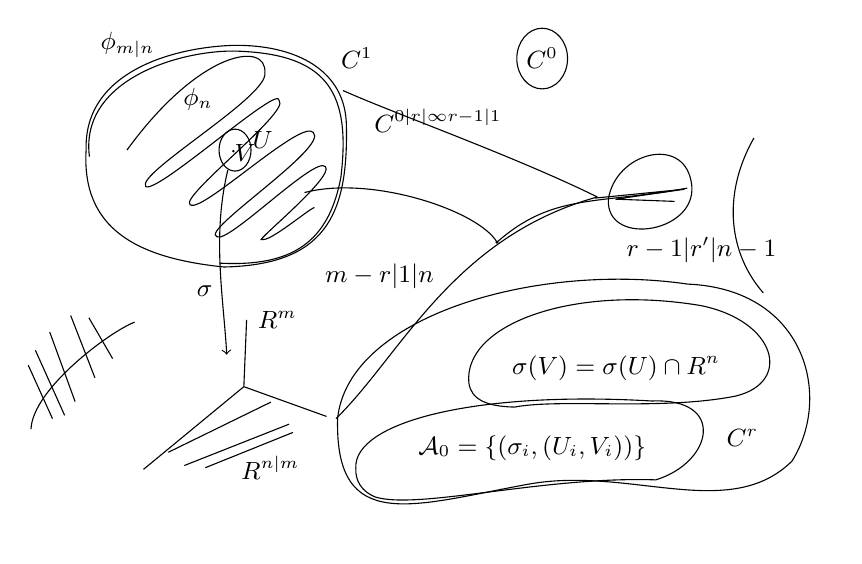
\begin{tikzpicture}[x=.007cm,y=-.007cm,every node/.style={inner sep=1pt,font=\small}]
\draw (313,277) .. controls (309,136) and (471,91) .. (582,88) .. controls (692,87) and (785,132) .. (785,236) .. controls (788,398) and (745,486) .. (563,490) .. controls (407,474) and (304,422) .. (313,277);
\draw[thin] (319,290) .. controls (300,144) and (500,92) .. (597,99) .. controls (753,107) and (793,177) .. (775,327) .. controls (753,445) and (687,490) .. (555,483);
\draw (387,278) .. controls (520,95) and (642,80) .. (637,138) .. controls (645,180) and (403,320) .. (421,344) .. controls (441,359) and (665,156) .. (663,188) .. controls (686,209) and (455,383) .. (508,378) .. controls (545,372) and (705,222) .. (725,246) .. controls (754,273) and (518,425) .. (550,435) .. controls (570,449) and (729,287) .. (747,308) .. controls (764,326) and (614,448) .. (632,440) .. controls (646,445) and (714,387) .. (727,382);
\draw (583,278) ellipse (29 and 38);
\fill (580,280) circle (2.5);
\node at (601,283) {$V$}; \node at (633,259) {$U$};
\node at (388,88) {$\phi_{\unsure{m|n}}$}; \node at (516,186) {$\phi_n$};
\node at (804,111) {$C^1$}; \node at (951,225) {$C^{\deleted{\unsure{0|r|\infty}}\unsure{r-1|1}}$};
\draw (1140,112) ellipse (46 and 55); \node at (1140,111) {$C^0$}; \node at (1266,132) {$\varnothing$};
\draw (709,355) .. controls (831,323) and (1025,388) .. (1058,445);
\fill (1058,445) circle (3); \draw (1058,445) .. controls (1159,356) and (1237,377) .. (1403,347);
\draw (766,765) .. controls (884,650) and (977,436) .. (1240,363);
\draw[thin] (779,170) .. controls (865,209) and (1090,289) .. (1240,363);
\draw (1260,367) .. controls (1273,283) and (1394,251) .. (1410,334) .. controls (1430,427) and (1255,457) .. (1260,367);
\draw (1236,365)--(1398,349)--(1273,367)--(1380,371); \draw (1524,256) .. controls (1465,360) and (1479,466) .. (1541,537); \node at (1429,459) {$\unsure{r-1|r'|n-1}$};
\node at (845,507) {$m-\unsure{r|1|n}$};
\draw[->] (570,314) .. controls (541,434) and (562,544) .. (568,649); \node at (528,534) {$\sigma$};
\draw (604,586)--(599,707)--(749,761); \draw (599,707)--(417,857);
\draw (462,826)--(648,735) (491,850)--(681,775) (529,854)--(688,790);
\node at (660,586) {$R^m$}; \node at (647,854) {$R^{\unsure{n|m}}$};
\draw[thin] (213,784) .. controls (216,711) and (356,607) .. (401,590);
\draw[thin] (208,668)--(252,765) (221,641)--(274,759) (247,608)--(293,734) (285,578)--(329,691) (318,582)--(361,656);
\draw (769,765) .. controls (788,578) and (1132,481) .. (1404,521) .. controls (1617,530) and (1667,724) .. (1593,842) .. controls (1479,954) and (1299,850) .. (1114,884) .. controls (906,922) and (764,976) .. (769,765);
\draw[thin] (1007,700) .. controls (997,594) and (1196,521) .. (1428,560) .. controls (1565,588) and (1594,699) .. (1491,724) .. controls (1355,751) and (1174,728) .. (1090,744) .. controls (1039,743) and (1011,730) .. (1007,700);
\node at (1274,673) {$\sigma(V)=\sigma(U)\cap R^n$};
\draw[thin] (802,855) .. controls (797,772) and (1016,714) .. (1339,733) .. controls (1474,727) and (1450,844) .. (1346,876) .. controls (1143,869) and (915,931) .. (837,907) .. controls (813,897) and (801,878) .. (802,855);
\node at (1122,818) {$\mathcal A_0=\{(\sigma_i,(U_i,V_i))\}$}; \node at (1503,800) {$C^r$};
\end{tikzpicture}}
% @ text / list of four families with right brace on its last two lines
\[
\begin{aligned}
&\boxed{1)\ \text{Familles canoniques}\quad C^r,\ r\geq0} && V_i\subset U_i\\
&2)\ \text{Familles régulières (quasi-régulières)},\ C^r,\ r\geq1\\
&\left.\begin{aligned}
3)&\ \text{familles naturelles}, &r\geq1\\
4)&\ \text{familles normales}, &r\geq1
\end{aligned}\right\}\ C^{r-1}
\end{aligned}
\]
% @ display / lower left, encircled pairs and conditions underneath
\[
\begin{aligned}
&\tikz[baseline=(p.base)]{\node[draw,ellipse,inner xsep=4pt,inner ysep=1.2pt] (p) {$(\sigma_1,(U_1,V_1))\qquad(\sigma_2,(U_2,V_2))$};}\\
1)\quad& V_1\cap V_2\neq\varnothing\\
2)\quad&(\sigma'_1,(U_1\cap U_2,V_1\cap V_2))\\
&\underline{(\sigma'_2,(U_1\cap U_2,V_1\cap V_2))}\\
&U_1\cap V_2=V_1\cap V_2\\
&U_2\cap V_1=V_1\cap V_2
\end{aligned}
\]
% @ drawing / lower right, overlapping patches and images under two arrows
\figure{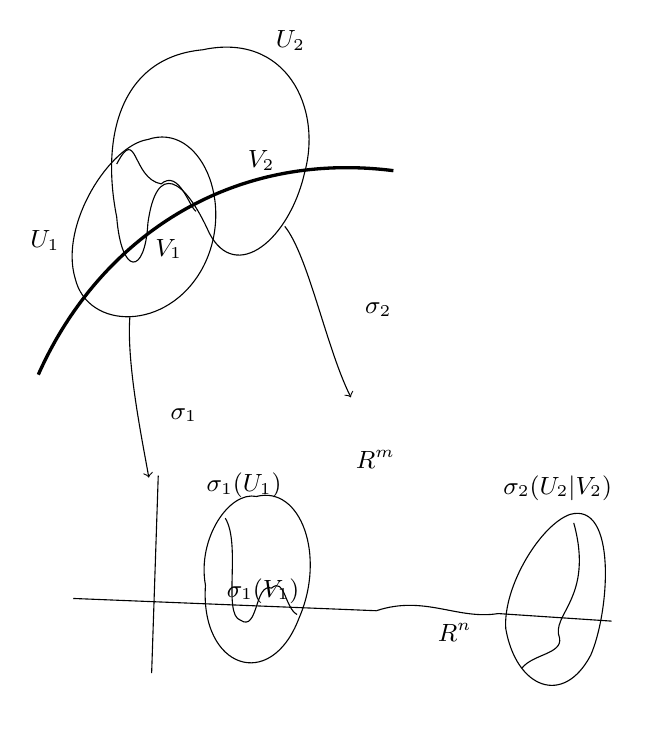
\begin{tikzpicture}[x=.012cm,y=-.012cm,every node/.style={inner sep=1pt,font=\small}]
\draw (1080,1537) .. controls (1063,1480) and (1117,1396) .. (1157,1390) .. controls (1212,1371) and (1251,1458) .. (1215,1526) .. controls (1178,1594) and (1093,1592) .. (1080,1537);
\draw (1124,1472) .. controls (1107,1387) and (1128,1303) .. (1215,1295) .. controls (1303,1276) and (1342,1356) .. (1323,1425) .. controls (1307,1496) and (1250,1543) .. (1222,1489) .. controls (1196,1431) and (1166,1412) .. (1157,1479) .. controls (1154,1534) and (1129,1535) .. (1124,1472);
\draw[very thick] (1041,1639) .. controls (1105,1495) and (1244,1401) .. (1417,1423);
\draw (1124,1416) .. controls (1146,1374) and (1140,1431) .. (1171,1437) .. controls (1190,1421) and (1201,1462) .. (1208,1466);
\node at (1048,1497) {$U_1$};\node at (1308,1285) {$U_2$};\node at (1179,1506) {$V_1$};\node at (1277,1412) {$V_2$};
\draw[->] (1138,1577) .. controls (1134,1628) and (1152,1713) .. (1158,1748);
\draw[->] (1302,1482) .. controls (1327,1513) and (1346,1611) .. (1372,1663);
\node at (1195,1682) {$\sigma_1$};\node at (1401,1570) {$\sigma_2$};
\draw (1168,1746)--(1161,1955) (1078,1876)--(1399,1889) (1528,1892)--(1648,1900);
\draw[thin] (1399,1889)..controls(1450,1872)and(1485,1899)..(1528,1892);
\draw (1218,1862) .. controls (1209,1813) and (1243,1762) .. (1272,1768) .. controls (1319,1756) and (1346,1831) .. (1317,1897) .. controls (1287,1976) and (1212,1950) .. (1218,1862);
\draw (1239,1791) .. controls (1256,1819) and (1236,1893) .. (1255,1899) .. controls (1274,1912) and (1270,1859) .. (1288,1865) .. controls (1302,1853) and (1302,1886) .. (1315,1893);
\draw (1536,1908) .. controls (1533,1863) and (1573,1798) .. (1604,1787) .. controls (1654,1773) and (1646,1890) .. (1626,1936) .. controls (1597,1991) and (1547,1971) .. (1536,1908);
\draw (1608,1796) .. controls (1630,1876) and (1583,1893) .. (1593,1918) .. controls (1596,1935) and (1564,1935) .. (1553,1950);
\node at (1398,1729) {$R^m$};\node at (1482,1912) {$R^n$};
\node at (1259,1756) {$\sigma_1(U_1)$};\node at (1279,1868) {$\sigma_1(V_1)$};\node at (1591,1759) {$\sigma_2(\unsure{U_2|V_2})$};
\end{tikzpicture}}
\scanpage{31}
% archive sheet number: 30
% @ text / opening question
$M=E_S\xrightarrow{u}E'_S=M'$ compatible avec
$\nabla_M,\inserted{\nabla_N,}F_{\deleted{\unsure{N|E}}M}\deleted{\unsure{?}},F_N$ ?
% @ display / upper two lines
\[
\begin{aligned}
u\circ A&=du+A'\circ u\\
&\boxed{du=u\circ A-A'\circ u}
\end{aligned}
\]
% @ diagram / square under equations, boxed identity at right
\diagram{\begin{tikzcd}[ampersand replacement=\&]
 E_S\arrow[r,"u"]\&E'_S\&\boxed{F_{M'}u^\sigma=uF_M}\\
 E_S\arrow[u,"F_M"]\arrow[r,"{F_S^*(u)=u^\sigma}"]\&E'_S\arrow[u,"F_{M'}"']\&
\end{tikzcd}}
% @ text / example, heading
\uline{Ex}\qquad \uline{Modules inversibles}. Alors
% @ display / scalar data and three boxed conditions
\[
\begin{aligned}
\Phi&=\varphi\in\Gamma(\underline O_S)\\
A&=\omega\in\Gamma(\widehat\Omega^1_{S/W})
\end{aligned}
\qquad
\boxed{\begin{aligned}
d\varphi&=\varphi(\omega^\sigma-\omega)\\
d\omega&=0\\
\varphi\psi&=p^{\unsure{N|n|i}}
\end{aligned}}
\]
% @ text / isomorphism condition
Si on a de $=$ $(\varphi',\omega')$, ils sont isom ssi $\exists\ u\in\Gamma O_S^{\unsure{*|\times}}$ satisfaisant
% @ display / struck condition and live two-line box
\[
\begin{aligned}
&\deleted{\unsure{d\omega|du}\ \frac{du}{u}=\omega-\omega'}\\
&\boxed{\left\{\begin{aligned}
\omega'-\omega&=-\frac{du}{u}\\
\varphi'/\varphi&=u/u^\sigma
\end{aligned}\right.}
\end{aligned}
\]
% @ text / conclusion above bottom diagram
Donc, classification est donnée par le défaut d'exactitude de
% @ diagram / final row and element formulas
\diagram{\begin{tikzcd}[ampersand replacement=\&,column sep=small]
\Gamma(\underline O_S^{\unsure{\times|*}})\arrow[r]\&
\Gamma(\deleted{\unsure{\Omega|2|\mathbb Z}}\widehat\Omega^1_{S/W})\times\Gamma(\underline O_S)^{!}\arrow[r]\&
\Gamma(\Omega^2_{S/W})\times\Gamma(\deleted{\unsure{\underline O_S|\Omega_S}}\Omega^1_S)[1/p]\\
u\arrow[r,mapsto]\&(-\frac{du}{u},u/u^\sigma)\&\\
\&(\varphi,\omega)\arrow[r]\&(d\omega,\frac{d\varphi}{\varphi}-(\omega^\sigma-\omega))
\end{tikzcd}}
% @ insertion / curved pointer from lower phi to small three-line gloss
\inserted{éléments inversibles dans $A[1/p]$}
\scanpage{32}
% sheet: reused_typed
% hand: typed
% archive sheet number: 31
% Typescript rotated 180 degrees relative to the archive foliation.
% @ handwritten / top centre in reading orientation
\handwritten{\mspage{55 \unsure{ter|der}}}
% @ text / proof, opening
\uline{Démonstration}. Le cas a) n'est autre que 5.10 et a été mis pour mémoire.
% @ text / proof, part b
b) \deleted{Le cas $\ell\neq p$ n'est autre que le critère galoisien de \unsure{la|ré}} \inserted{La première assertion est une conséquence \deleted{immé} triviale de} a) et des définitions. Pour prouver la dernière assertion dans b), on peut \deleted{donc} supposer que $\ell\neq p$, mais alors grâce à a) il suffit de prendre pour $K'$ une extension finie séparable de $K$ correspondant à un sous-groupe ouvert $\handwritten{\pi'}$ de $\handwritten{\pi}=\mathrm{Gal}(\bar K/K)$ dont l'intersection avec le groupe d'inertie $I$ est contenue dans le \deleted{stabli} noyau de la représentation de $I$ sur $T_{\ell}(A_K(\bar K))$, lequel est \deleted{\unsure{fi|à}} ouvert par hypothèse (cf. 5.12.1).
% @ text / proof, first three implications
c) On a déjà signalé que $1)\handwritten{\Rightarrow}2)$ (5.12.2), il est trivial que $2)\handwritten{\Rightarrow}3)$, reste à prouver que $3)\handwritten{\Rightarrow}1)$. Pour $\ell\neq p$, ce n'est autre que \inserted{le} cri\deleted{\unsure{t|i}}tère galoisien de réduction semi-stable 3.5. Pour $\ell=p$, on peut procéder ainsi. \deleted{\unsure{A|O}}Choisissons un nombre premier $\ell'\neq p$, et appliquons à celui-ci les considérations d e 4.1. \deleted{On est donc ramené à prouver que la représentation}
% @ text / proof, strictly local case through end
Supposons $S$ strictement local, ce qui est loisible (3.4.0), prenons une extension galoisienne finie $K'$ de $K$, d\deleted{d}e groupe $G$, telle que $A_{K'}$ ait réduction semi-stable. Il faut prouver que la représentation de $G$ sur les trois quotients intervenant dans (4.1.1) est triviale, ou ce qui revient au même, que la \deleted{somme des traces} représentation somme est triviale, ou encore, que la trace de cette dernière est "triviale", i.e. constante . Or nous avons vu dans 4.3 a) que cette fonction trace est indépendante d\deleted{\unsure{a}}u choix de $\ell'\neq p$, et dans 6.\deleted{\unsure{6|5}}\handwritten{4} plus bas nous indiquons une méthode de calcul de cette fonction en \deleted{fonction}\inserted{termes} de $T_p(A_K)$ également. Ce calcul donne trivialement une fonction constante dans le cas où $T_p(A_K)$ a bonne réduction virtuelle, et cela achève la démonstration.
% @ text / bottom, remark, with inserted qualifier and manuscript postscript
\uline{Remarque} 5.13.1. Il semble plausible que si $X_{\handwritten{\eta}}$ est un \handwritten{\inserted{pro-$\unsure{l|\ell}$-}}groupe de Barsotti-Tate sur $\handwritten{\eta}$ qui a bonne réduction virtuelle sur $S$, et bonne réduction virtuelle essentielle d'échelon $n$, alors il a \deleted{\unsure{v|b}}bonne réduction virtuelle d'échelon $n$. \handwritten{(C'est \deleted{ce qui avait été utilisé, pour} vrai pour $l\neq p$.)}
\scanpage{34}
% archive sheet number: 33
% @ text / title, two lines
Détermination du module de Dieudonné filtré du groupe de Lubin-Tate.
% @ text / field and valuation ring
$K$ extension finie de $\mathbb Q_p$, anneau d'entiers $A$, corps résiduel
% @ diagram / square and data on its right
\diagram{\begin{tikzcd}[ampersand replacement=\&]
\mathbb Z_p\arrow[r,dash]\arrow[d,dash]\&A\arrow[d,dash]\& k\simeq\mathbb F_q,\ q=p^f\\
\mathbb Q_p\arrow[r,dash]\&K\&{[K:\mathbb Q_p]=h=ef}\\
\&\&\pi\in A\quad\text{uniformisante}
\end{tikzcd}}
% @ text / Witt vectors
$W=W_\infty(k)$ vecteurs de Witt,
% @ diagram / two inclusions with parenthesized degrees
\diagram{\begin{tikzcd}[ampersand replacement=\&]
\mathbb Z_p\arrow[r,hook,"{(f)}"']\& W\arrow[r,hook,"i","{(e)}"']\& A
\end{tikzcd}}
% @ text / aim, with two words entered above the line
On veut déterminer \inserted{d'abord} les groupes de B.T. \inserted{$G_0$} de hauteur $(=\unsure{\mathrm{rang}|v.\,\mathrm{g}})$ $h$ sur $\deleted{\unsure{\mathbb F_q|A|k}}\,k$, avec opération de $A$ dessus [telle que $\pi_{G_0}=F^f$ (automorphisme de Frobenius de $G_0/\mathbb F_q$)]
% @ text / Dieudonné theory, module and endomorphism
Par la théorie de Dieudonné, ils correspondent aux modules libres \inserted{$M$} de rang $h$ sur $W$, avec un endom $\sigma$-linéaire ($\sigma$ autom de Frob. de $W$) $F_M$, et opération de $A$ sur $M$ $(\lambda\mapsto\lambda_M)$ par $W$-\unsure{autom|endom} commutant à $F_M$, satisfaisant
% @ diagram / square on the left of the module conditions
\diagram{\begin{tikzcd}[ampersand replacement=\&]
A\arrow[r,dash]\arrow[d,dash]\& A\otimes_{\mathbb Z_p}W\arrow[d,dash]\\
\mathbb Z_p\arrow[r,dash]\&W
\end{tikzcd}}
% @ display / two starred requirements
\[
\left[(*)\qquad\deleted{\unsure{\pi_M|\lambda_M|\lambda_\pi}}\ F_M^f=\pi_{\underline M}\right]
\qquad
\begin{aligned}
(*')\quad&\exists\,V_M\ \text{t.q.}\\
&F_MV_M=V_MF_M=p
\end{aligned}
\]
% @ text / the two module structures
Les deux structures de module sur $M$ correspondent à une structure de module sur $A_W=A\otimes_{\mathbb Z_p}W$. Soit $\deleted{\unsure{F_{\mathbb Z_p}|F_W|\sigma_W}}\,\sigma_A$ l'autom de $A_W=A\otimes_{\mathbb Z_p}W$ donné par
% @ display / action on a simple tensor
\[
\sigma_A(\lambda\otimes w)=\lambda\otimes\sigma w
\]
% @ text / last two lines
Alors la donnée de $F_M$ équivaut à la donnée d'un endom $\sigma_A$-linéaire, satisfaisant $(*)\ (*')$.
